\newpage
\usecasebase{Modifica della propria ordinazione}
\label{usecase:Modifica della propria ordinazione}

\begin{figure}[h]
	\centering
	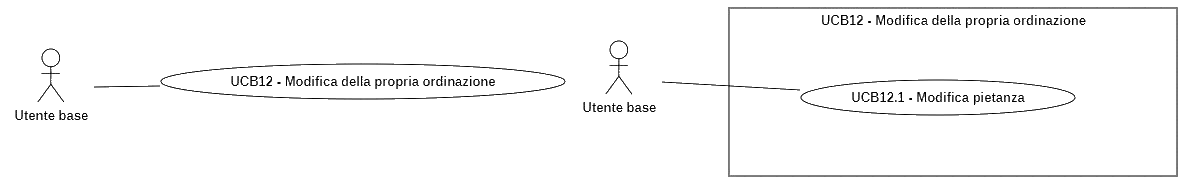
\includegraphics[width=0.99\textwidth]{./uml/UCB12.png} 
	\caption{Modifica dell'ordinazione collaborativa dei pasti}
	\label{fig:UCBmod_ord}
  \end{figure}

\begin{itemize}
	\item \textbf{Attore principale:} Utente base.

	\item \textbf{Precondizione:}
	      \begin{itemize}
		      \item L'Utente base sta effettuando un ordinazione collaborativa dei pasti (vedi \autoref{usecase:Creazione dell'ordinazione collaborativa dei pasti});
		      \item L'utente base deve rispettare un limite temporale: se vuole modificare il proprio ordine deve farlo ventiquattro ore prima a partire dall'ora stabilita della prenotazione.
	      \end{itemize}

	\item \textbf{Postcondizioni:}
	      \begin{itemize}
		      \item L'Utente base ha modificato il proprio ordine.
		      \item Il Sistema aggiorna le informazioni inerenti al suo ordine.
	      \end{itemize}

	\item \textbf{Scenario principale:}
	      \begin{enumerate}
		      \item L'Utente base modifica una propria pietanza (vedi \autoref{usecase:Modifica pietanza});
		      \item L'Utente base conferma il proprio ordine;
		      \item Il Sistema aggiorna il riepilogo dell'ordinazione.
	      \end{enumerate}
\end{itemize}

\subusecasebase{Modifica pietanza}
\label{usecase:Modifica pietanza}
\begin{itemize}
	\item \textbf{Attore principale:} Utente base.

	\item \textbf{Precondizioni:}  L'Utente base si trova nella sezione "Modifica della propria ordinazione" (vedi \autoref{usecase:Modifica della propria ordinazione}).


	\item \textbf{Postcondizione:} L'Utente base ha modificato una pietanza.

	\item \textbf{Scenario principale:}
	      \begin{enumerate}
		      \item L'Utente base seleziona tra le pietanze del suo ordine una che vuole modificare, ovvero:
		            \begin{itemize}
			            \item Modifica della quantità della pietanza selezionata.
			            \item Rimozione di ingredienti della pietanza selezionata.
		            \end{itemize}
		      \item L'Utente base conferma la sua modifica;
		      \item Il Sistema registra la sua modifica.
	      \end{enumerate}
\end{itemize}